\documentclass[aspectratio=169,xcolor=table]{beamer}
\usepackage{algorithm}
\usepackage{algpseudocode}
\usepackage[utf8]{inputenc}
\usepackage[T1]{fontenc}
\usepackage{lipsum, lmodern}
\usepackage{csquotes}
\usepackage{xcolor}
\usepackage[portuguese]{babel}
\usepackage{amsmath}
\usepackage{physics}

% ------------------------------------------------
% Tema do Beamer (exemplo de um tema customizado)
% ------------------------------------------------
\usetheme{DCC} % <-- Ajuste conforme seu tema ou estilo

\graphicspath{{imgs/}{./imgs/}}

\author[Magalhães, Felipe]{%
  \textbf{Antoniel Magalhães} \\
  \textbf{Luis Felipe}
}
\title{Simulação de ondas e oceano}
\institute{Universidade Federal da Bahia \\ Instituto de Computação}
\date{\today}

\begin{document}

%-------------------------------------------------
%  SLIDE DE TÍTULO
%-------------------------------------------------
\begin{frame}[plain,noframenumbering]
    \titlepage
\end{frame}

%-------------------------------------------------
%  SLIDE DE AGENDA
%-------------------------------------------------
\begin{frame}{Agenda}
    \tableofcontents
\end{frame}

\setlength{\parskip}{1em} % Adjust the space between paragraphs

%=================================================
\section{Introdução}
%=================================================
\begin{frame}{Introdução}
    \begin{itemize}
        \item A simulação de ondas e oceano é uma área de estudo que combina física, matemática e computação para modelar o comportamento das ondas no mar.
        \item Este campo é crucial para:
        \begin{itemize}
            \item Jogos e aplicações interativas
            \item Efeitos visuais em filmes e animações
            \item Visualização científica
            \item Simuladores de treinamento marítimo
        \end{itemize}
    \end{itemize}
\end{frame}

%=================================================
\section{Imagens dos Artigos de Referência}
%=================================================
\begin{frame}{Imagens dos Artigos de Referência}
    \begin{columns}
        \column{0.45\textwidth}
        \centering
        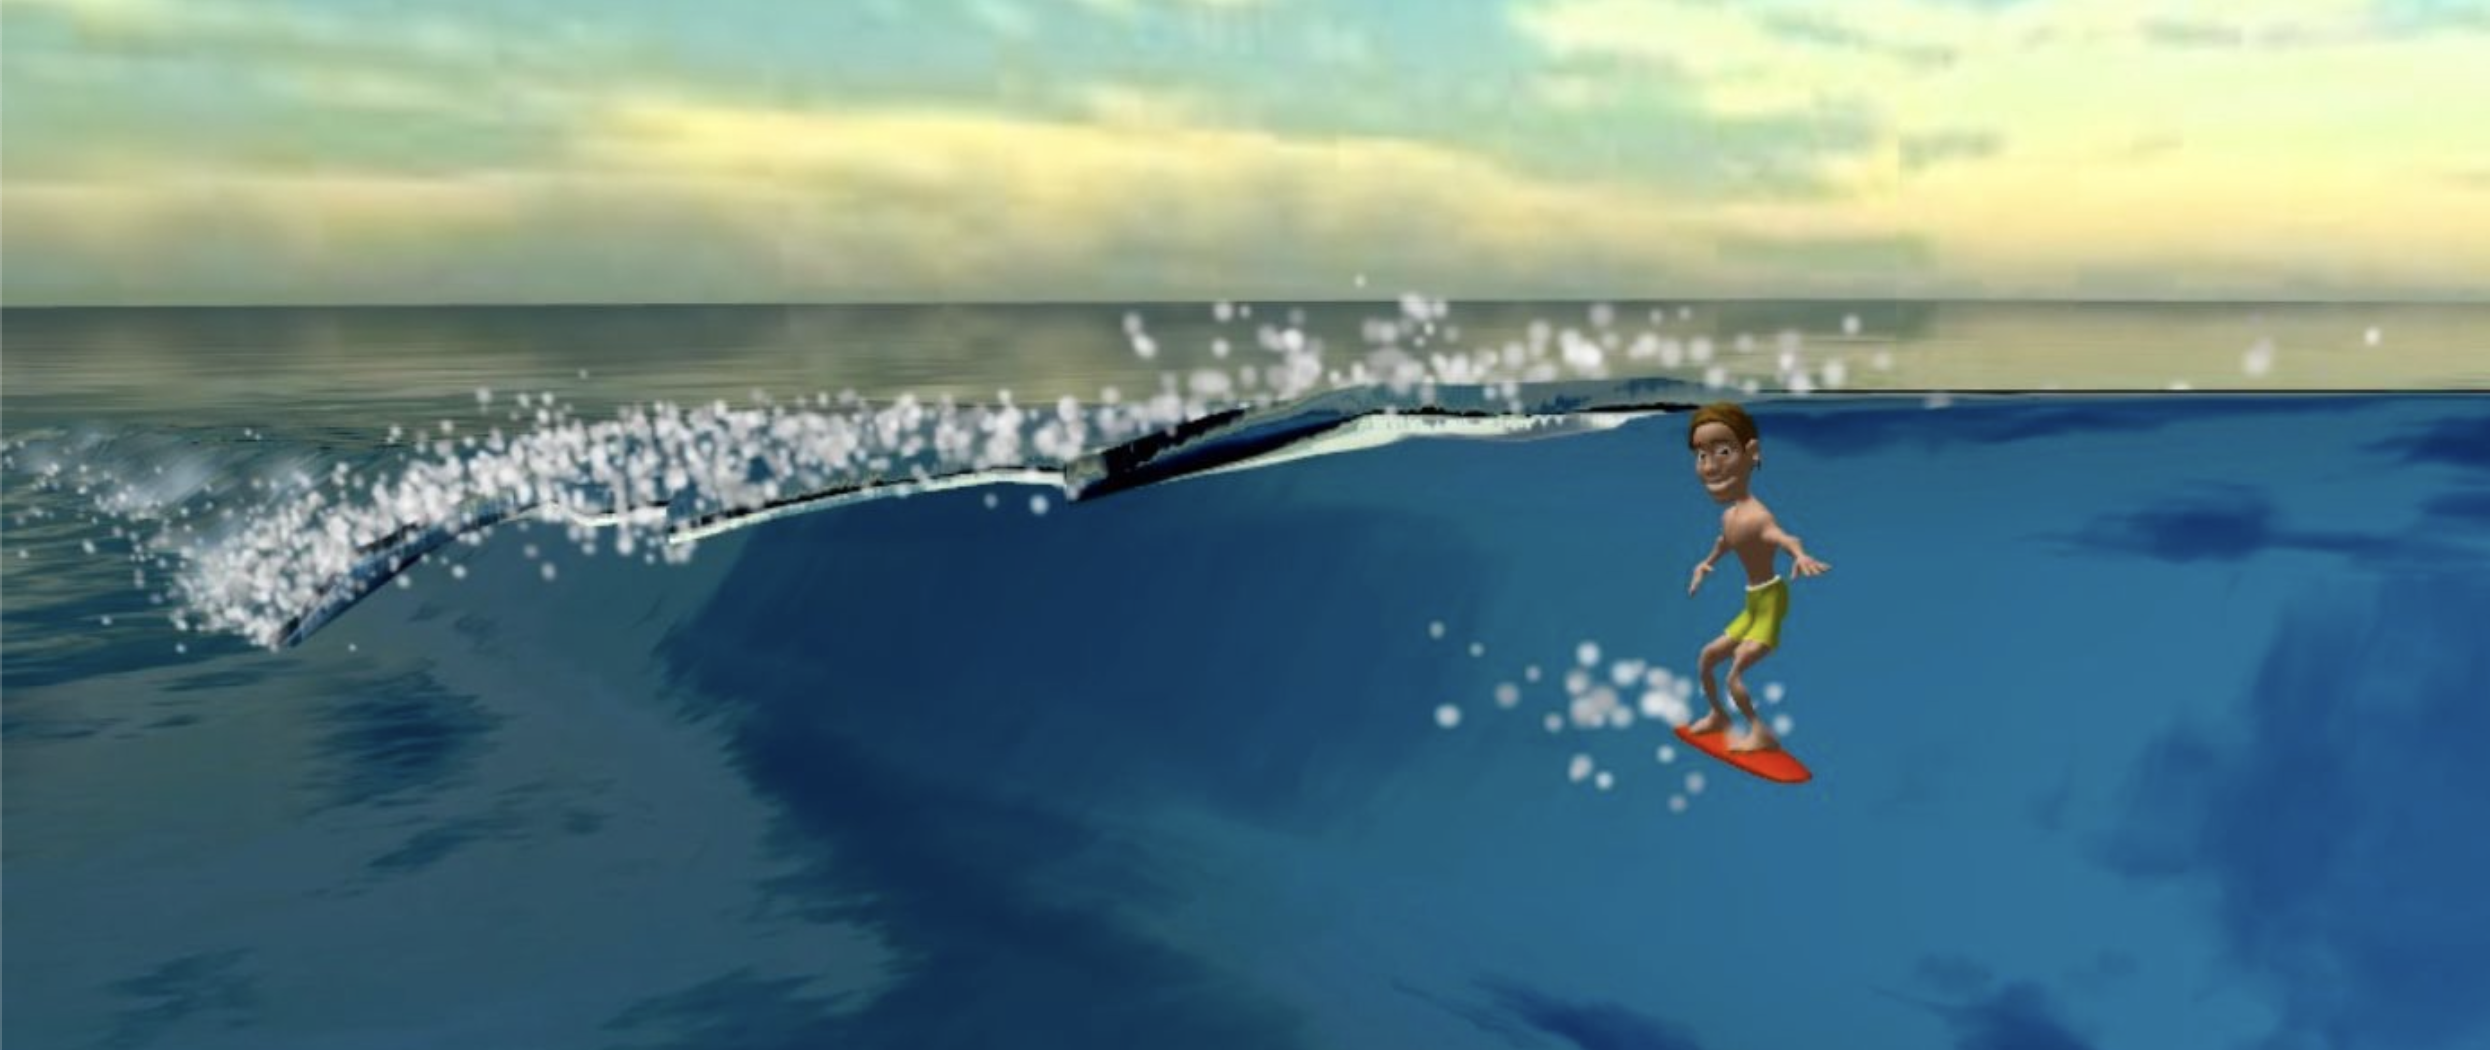
\includegraphics[width=\textwidth]{imgs/wave-artigo-1.png}
        
        \column{0.45\textwidth}
        \centering
        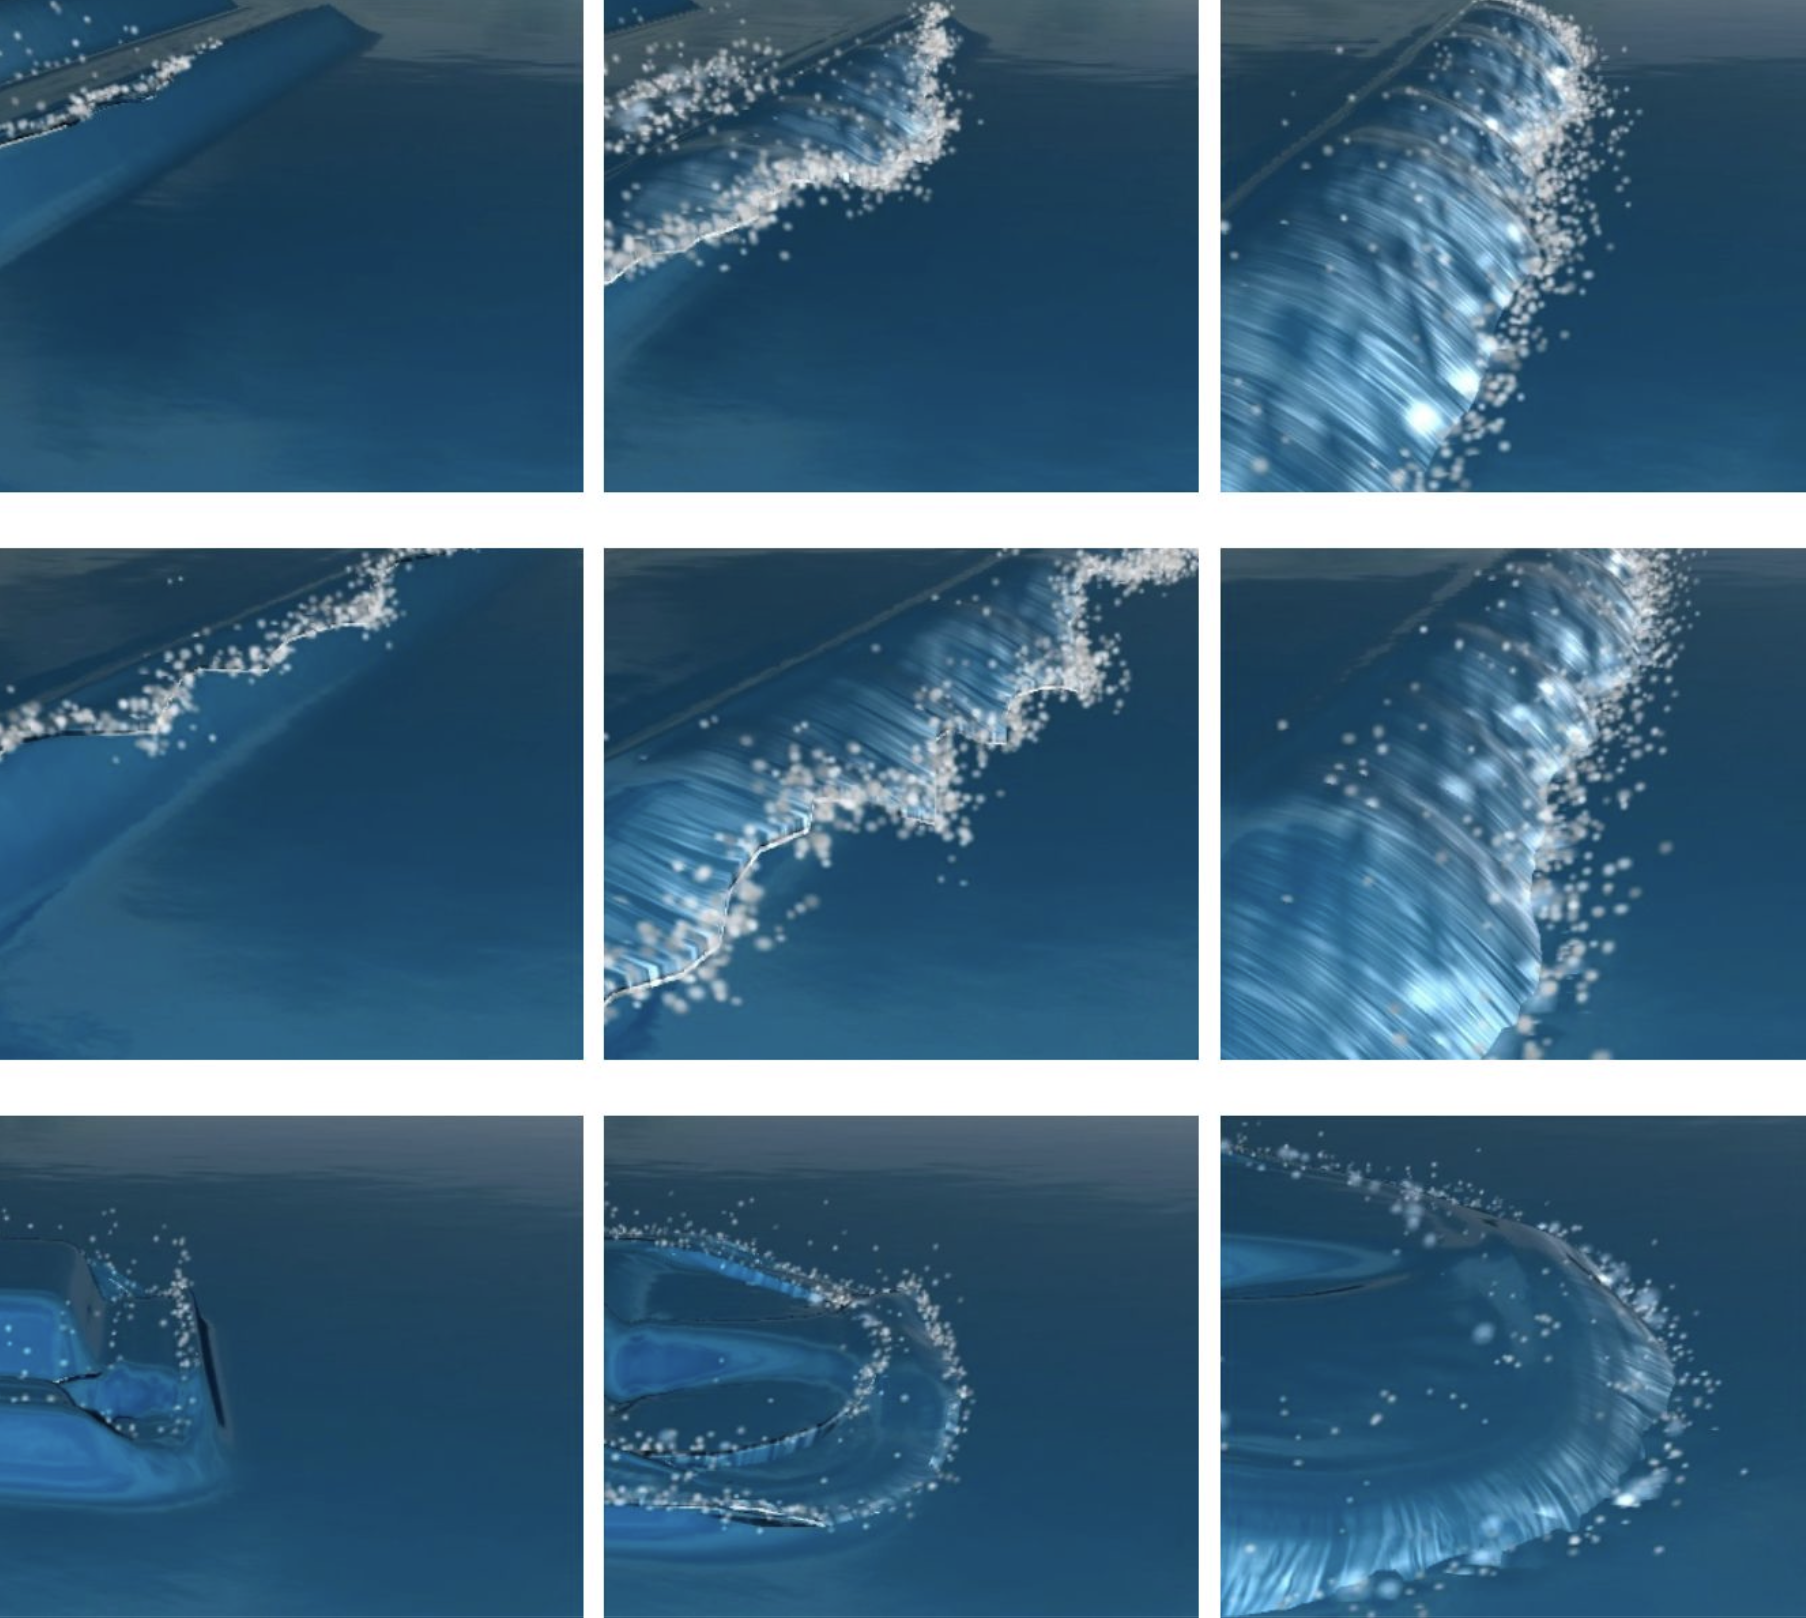
\includegraphics[width=\textwidth]{imgs/wave-artigo-2.png}
    \end{columns}
\end{frame}


%=================================================
\section{Computação Atual de Ondas}
%=================================================
\begin{frame}{Computação Atual de Ondas}
    \begin{columns}
        \column{0.45\textwidth}
        \centering
        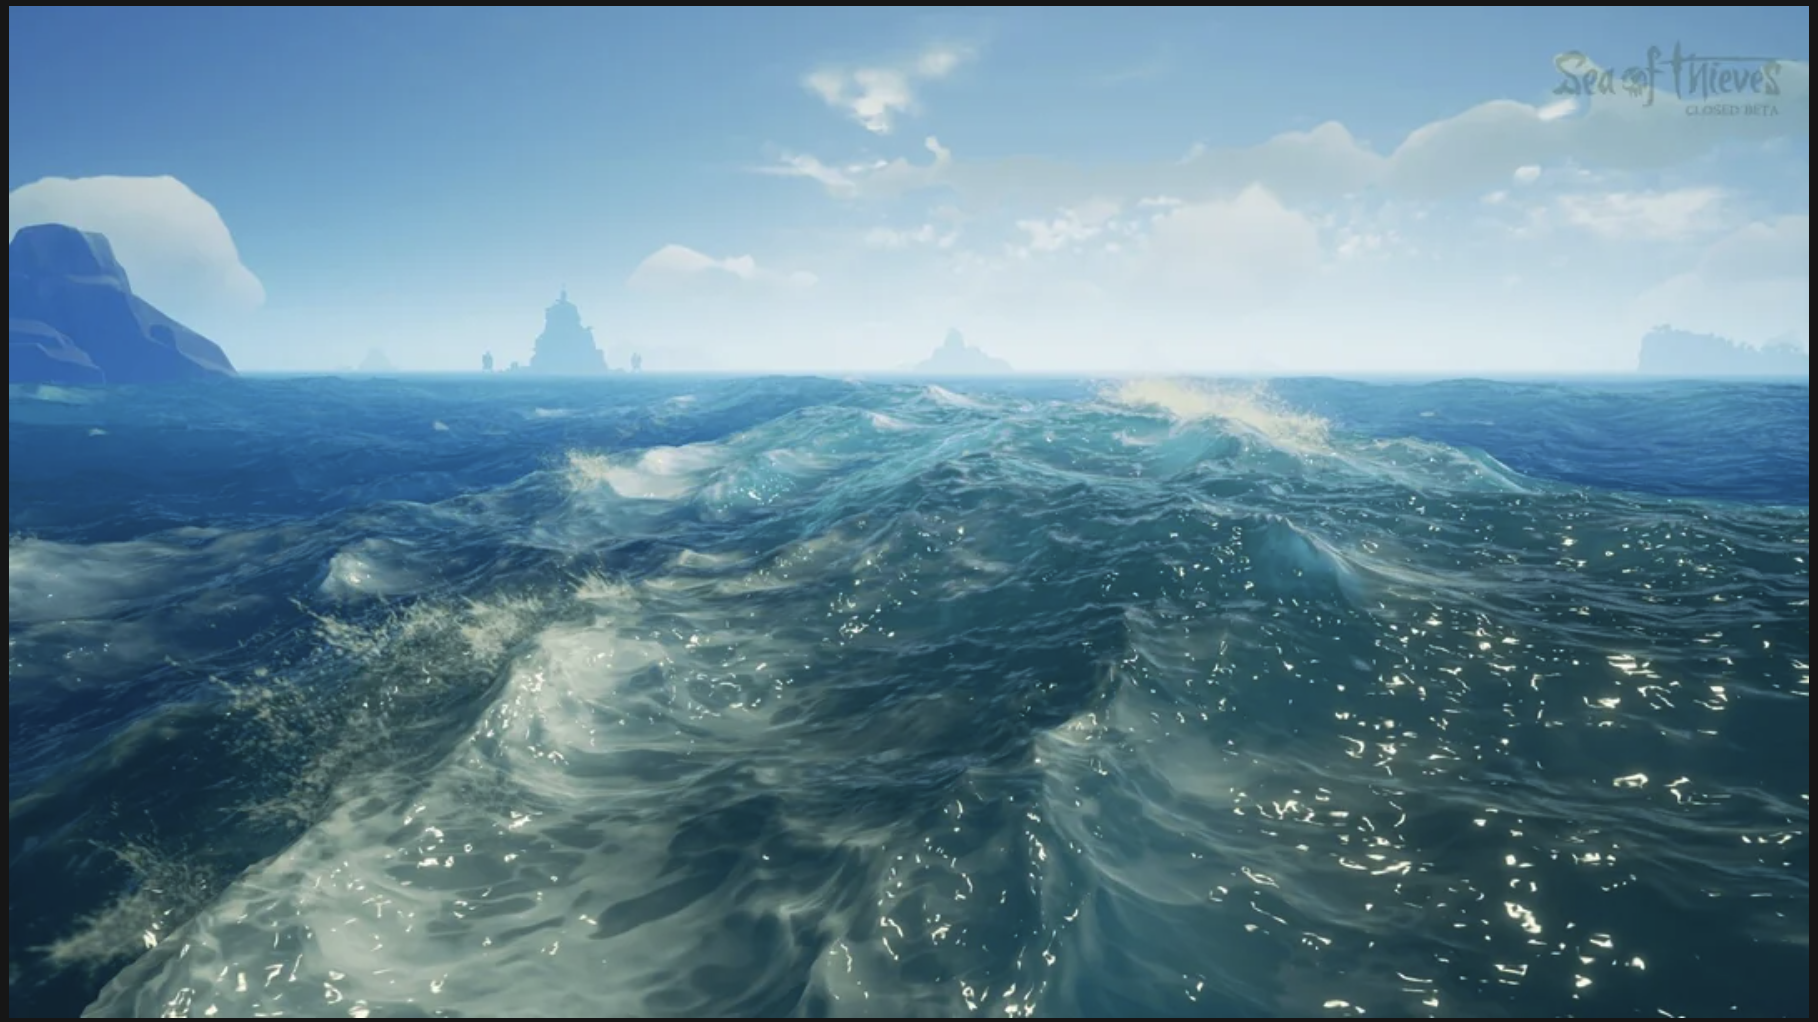
\includegraphics[width=\textwidth]{imgs/sea-of-thieves.png}
        
        \column{0.45\textwidth}
        \centering
        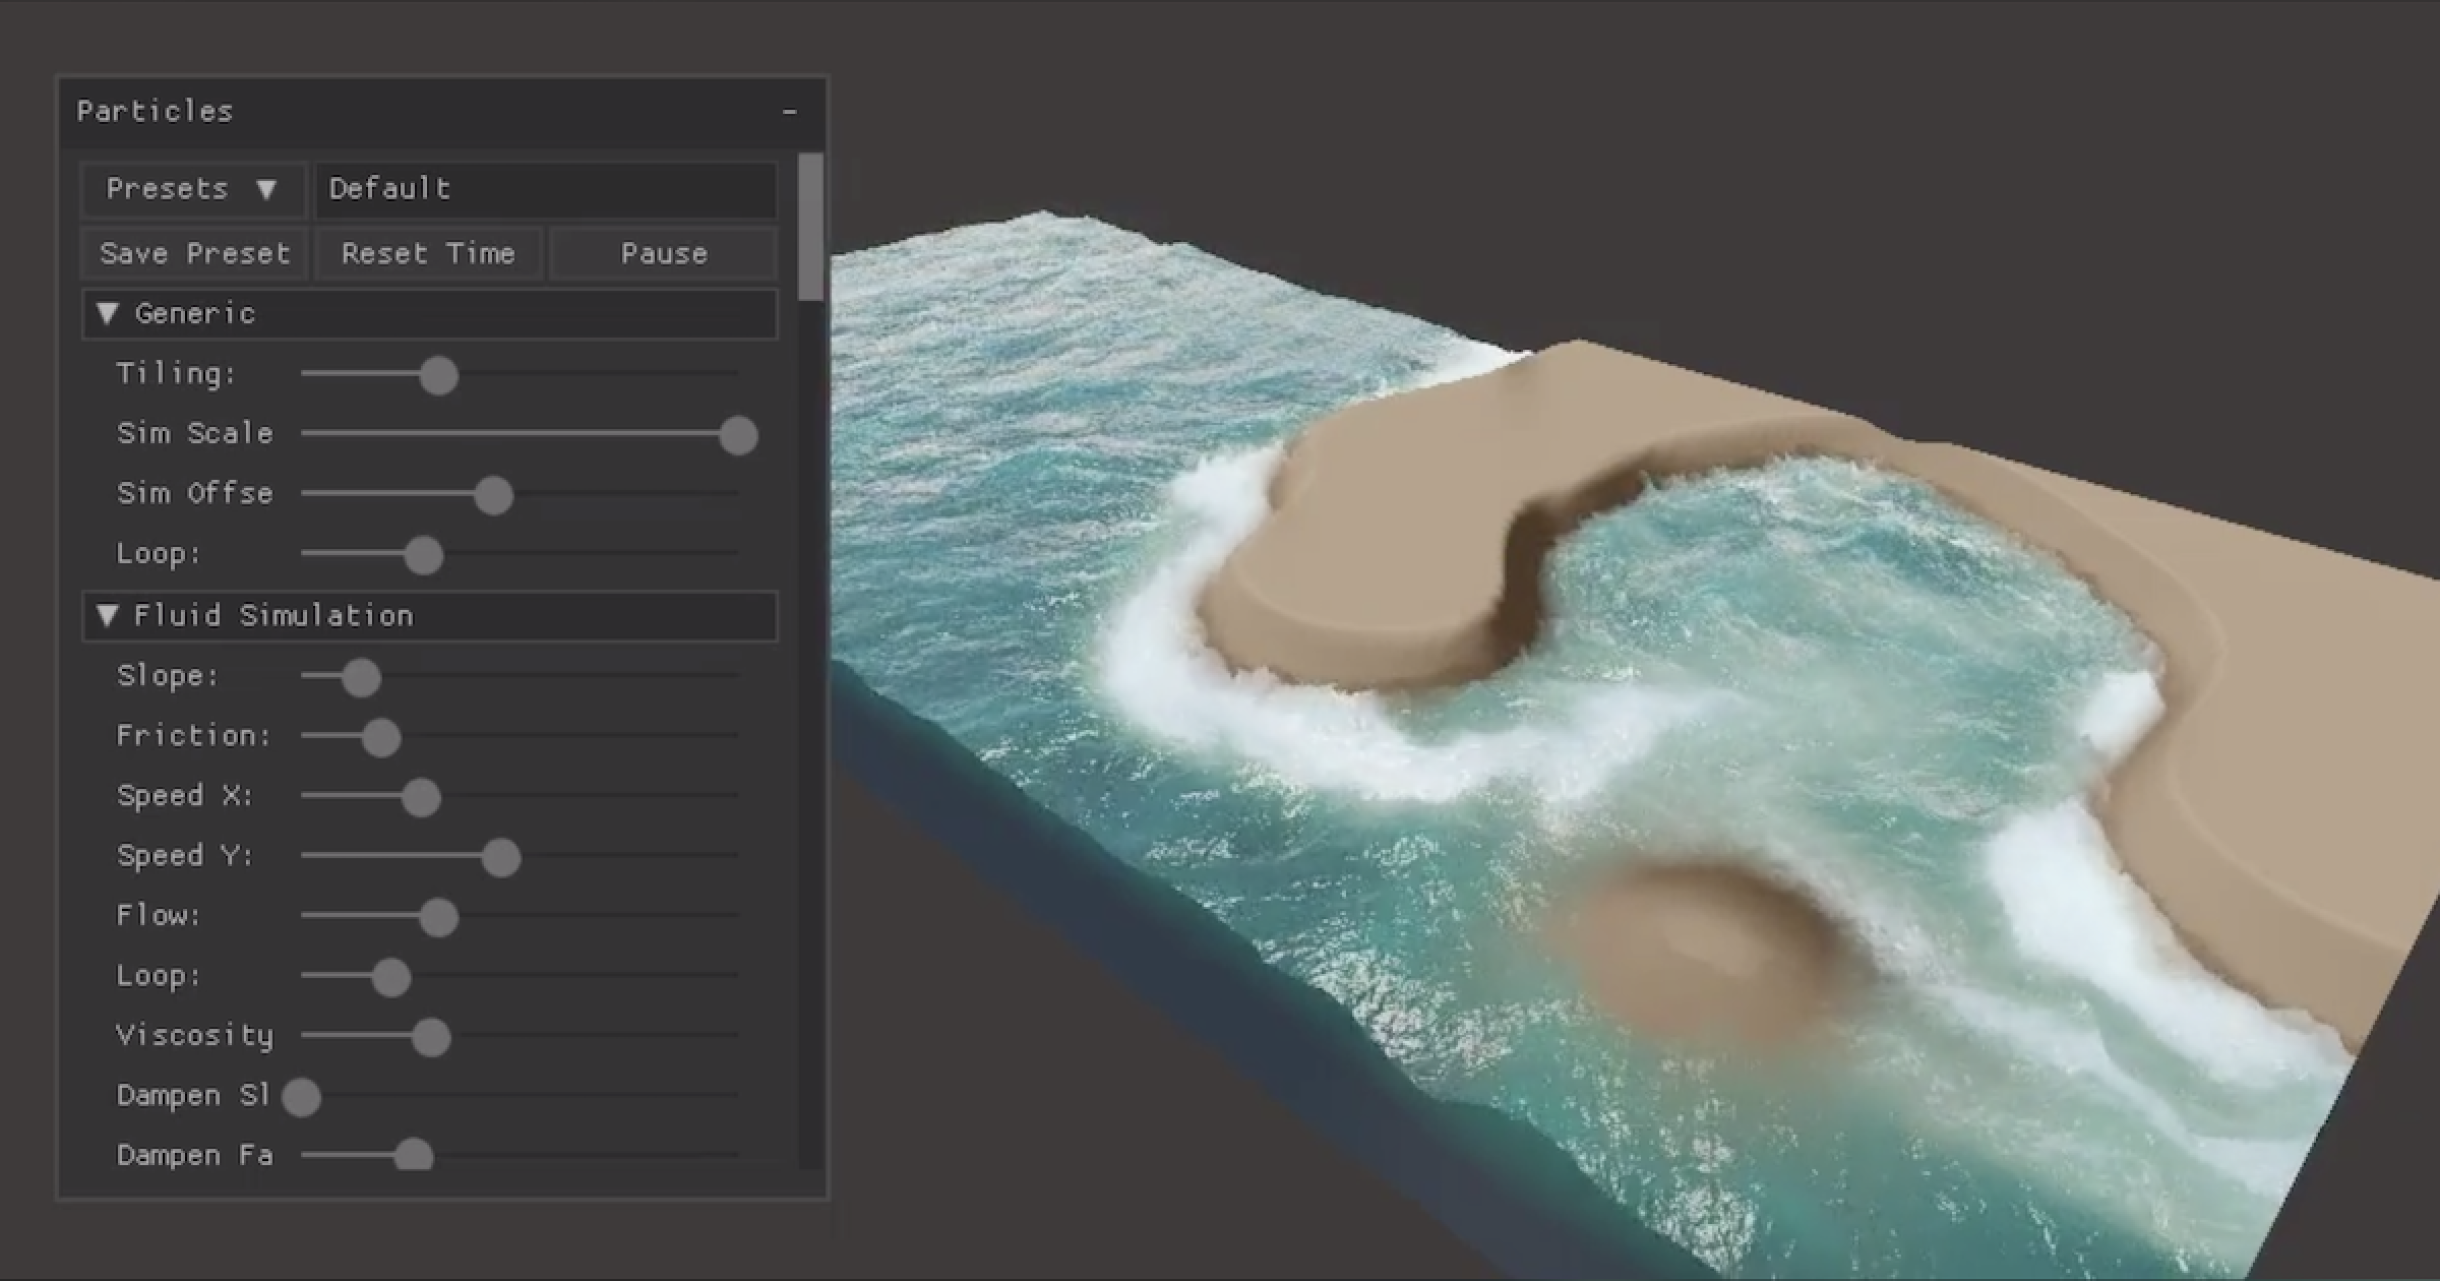
\includegraphics[width=\textwidth]{imgs/river-editor.png}
    \end{columns}
\end{frame}


\begin{frame}{Demonstração da Simulação}
    \begin{columns}
        \column{0.45\textwidth}
        \centering
        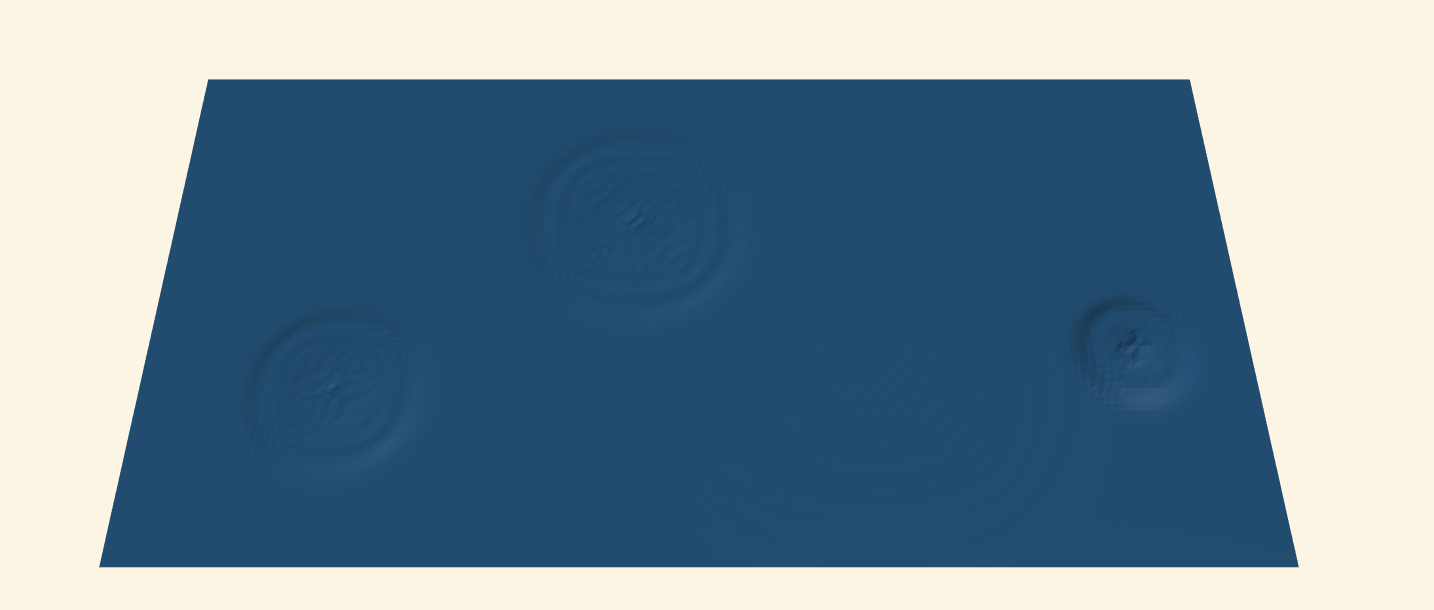
\includegraphics[width=\textwidth]{imgs/wave.png}
        
        \column{0.45\textwidth}
        \centering
        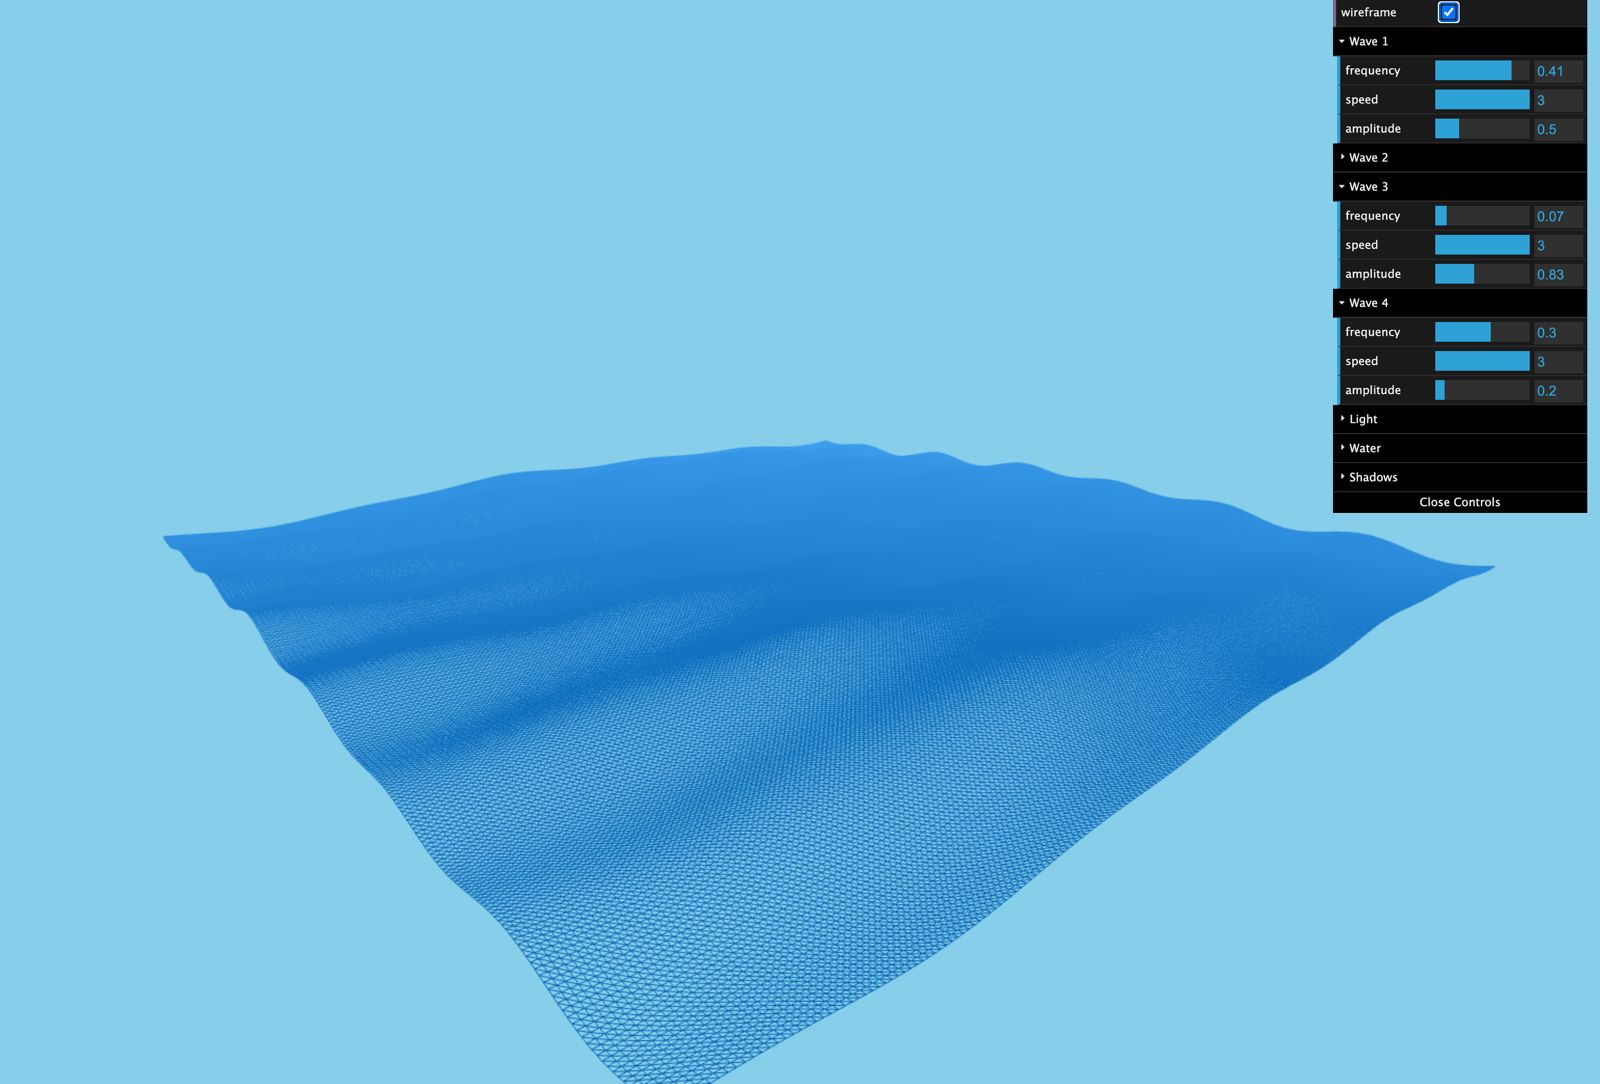
\includegraphics[width=\textwidth]{imgs/wave-2.jpeg}
    \end{columns}
\end{frame}


%=================================================
\section{Técnicas Avançadas de Simulação}
%=================================================
\begin{frame}{Survey: Estado da Arte em Simulação de Oceanos}
    \begin{itemize}
        \item \textbf{Simulação de Águas Profundas:}
        \begin{itemize}
            \item Abordagens \textbf{Espaciais}: funções periódicas
            \item Abordagens \textbf{Espectrais}: transformada de Fourier a partir de espectros de ondas
            \item Abordagens \textbf{Híbridas}: combinação dos métodos espaciais e espectrais
        \end{itemize}
        \item \textbf{Simulação de Águas Rasas:}
        \begin{itemize}
            \item Métodos \textbf{Eulerianos}: baseados nas equações de Navier-Stokes (NSE)
            \item Métodos \textbf{Lagrangianos}: por exemplo, Smoothed Particle Hydrodynamics (SPH)
            \item Métodos \textbf{Híbridos}: integração de abordagens Eulerianas e Lagrangianas
        \end{itemize}
    \end{itemize}
\end{frame}
\begin{frame}{Terrain and Water Rendering with Hardware Tessellation (2010)}
    \begin{itemize}
      \item \textbf{O que é Tesselação?}
        \begin{itemize}
          \item Técnica que subdivide a geometria na GPU em tempo real
          \item Gera níveis de detalhe adaptativos sem sobrecarregar a CPU
        \end{itemize}
      \item \textbf{Aplicações:}
        \begin{itemize}
          \item \textbf{Terrenos:} Renderização de superfícies extensas com detalhes variáveis
          \item \textbf{Oceanos:} Simulação de ondas com movimento físico e reflexões Fresnel
        \end{itemize}
      \item \textbf{Relação com o Survey:}
        \begin{itemize}
          \item Complementa métodos de geração de ondas (funções periódicas, Fourier)
          \item Utiliza tesselação para gerar geometrias detalhadas de ondas
        \end{itemize}
      \item \textbf{Resultados:}
        \begin{itemize}
          \item Melhor desempenho e realismo em cenas complexas
        \end{itemize}
    \end{itemize}
  \end{frame}

  \begin{frame}{Função Procedural para Geração de Ondas}
    \footnotesize
        \begin{itemize}
            \item \textbf{Objetivo:} Criar uma superfície ondulada realista aplicando deslocamentos a cada vértice.
            \item \textbf{Fórmula do Deslocamento:}
                \[
                s(p, a, \lambda, k, t) = a \begin{bmatrix} -\cos(\phi) \\ \sin(\phi) \end{bmatrix} \quad \text{com} \quad \phi = \frac{2\pi}{\lambda}(p\cdot k + v\,t)
                \]
            \item \textbf{Combinação de Ondas:}
                \[
                p_\Sigma = p + \sum_{i=0}^{n} s(p, a_i, \lambda_i, k_i, t)
                \]
            \item \textbf{Onde:}
                \begin{itemize}
                    \item \textbf{\(p\)} é a posição original do vértice, \textbf{\(a\)} é a amplitude da onda, \textbf{\(\lambda\)} é o comprimento de onda, \textbf{\(k\)} é a direção da onda (normalizada), \textbf{\(v\)} é a velocidade da onda e \textbf{\(t\)} é o tempo.
                \end{itemize}
            \item \textbf{Processo:} 
                \begin{itemize}
                    \item Aplicada a cada vértice da malha subdividida pela tesselação.
                    \item Executada no \textbf{Domain Shader}, onde os novos vértices são posicionados.
                \end{itemize}
            \item \textbf{Relação com o Survey:} 
                \begin{itemize}
                    \item Aqui, a tesselação gera dinamicamente os vértices, e a função procedural os transforma em uma geometria ondulada.
                \end{itemize}
        \end{itemize}
    \end{frame}

\begin{frame}{Demonstração}
    \begin{columns}
        \column{0.45\textwidth}
        \centering
        \includegraphics[width=\textwidth]{imgs/terrain-and-water.png}
        
        \column{0.45\textwidth}
        \centering
        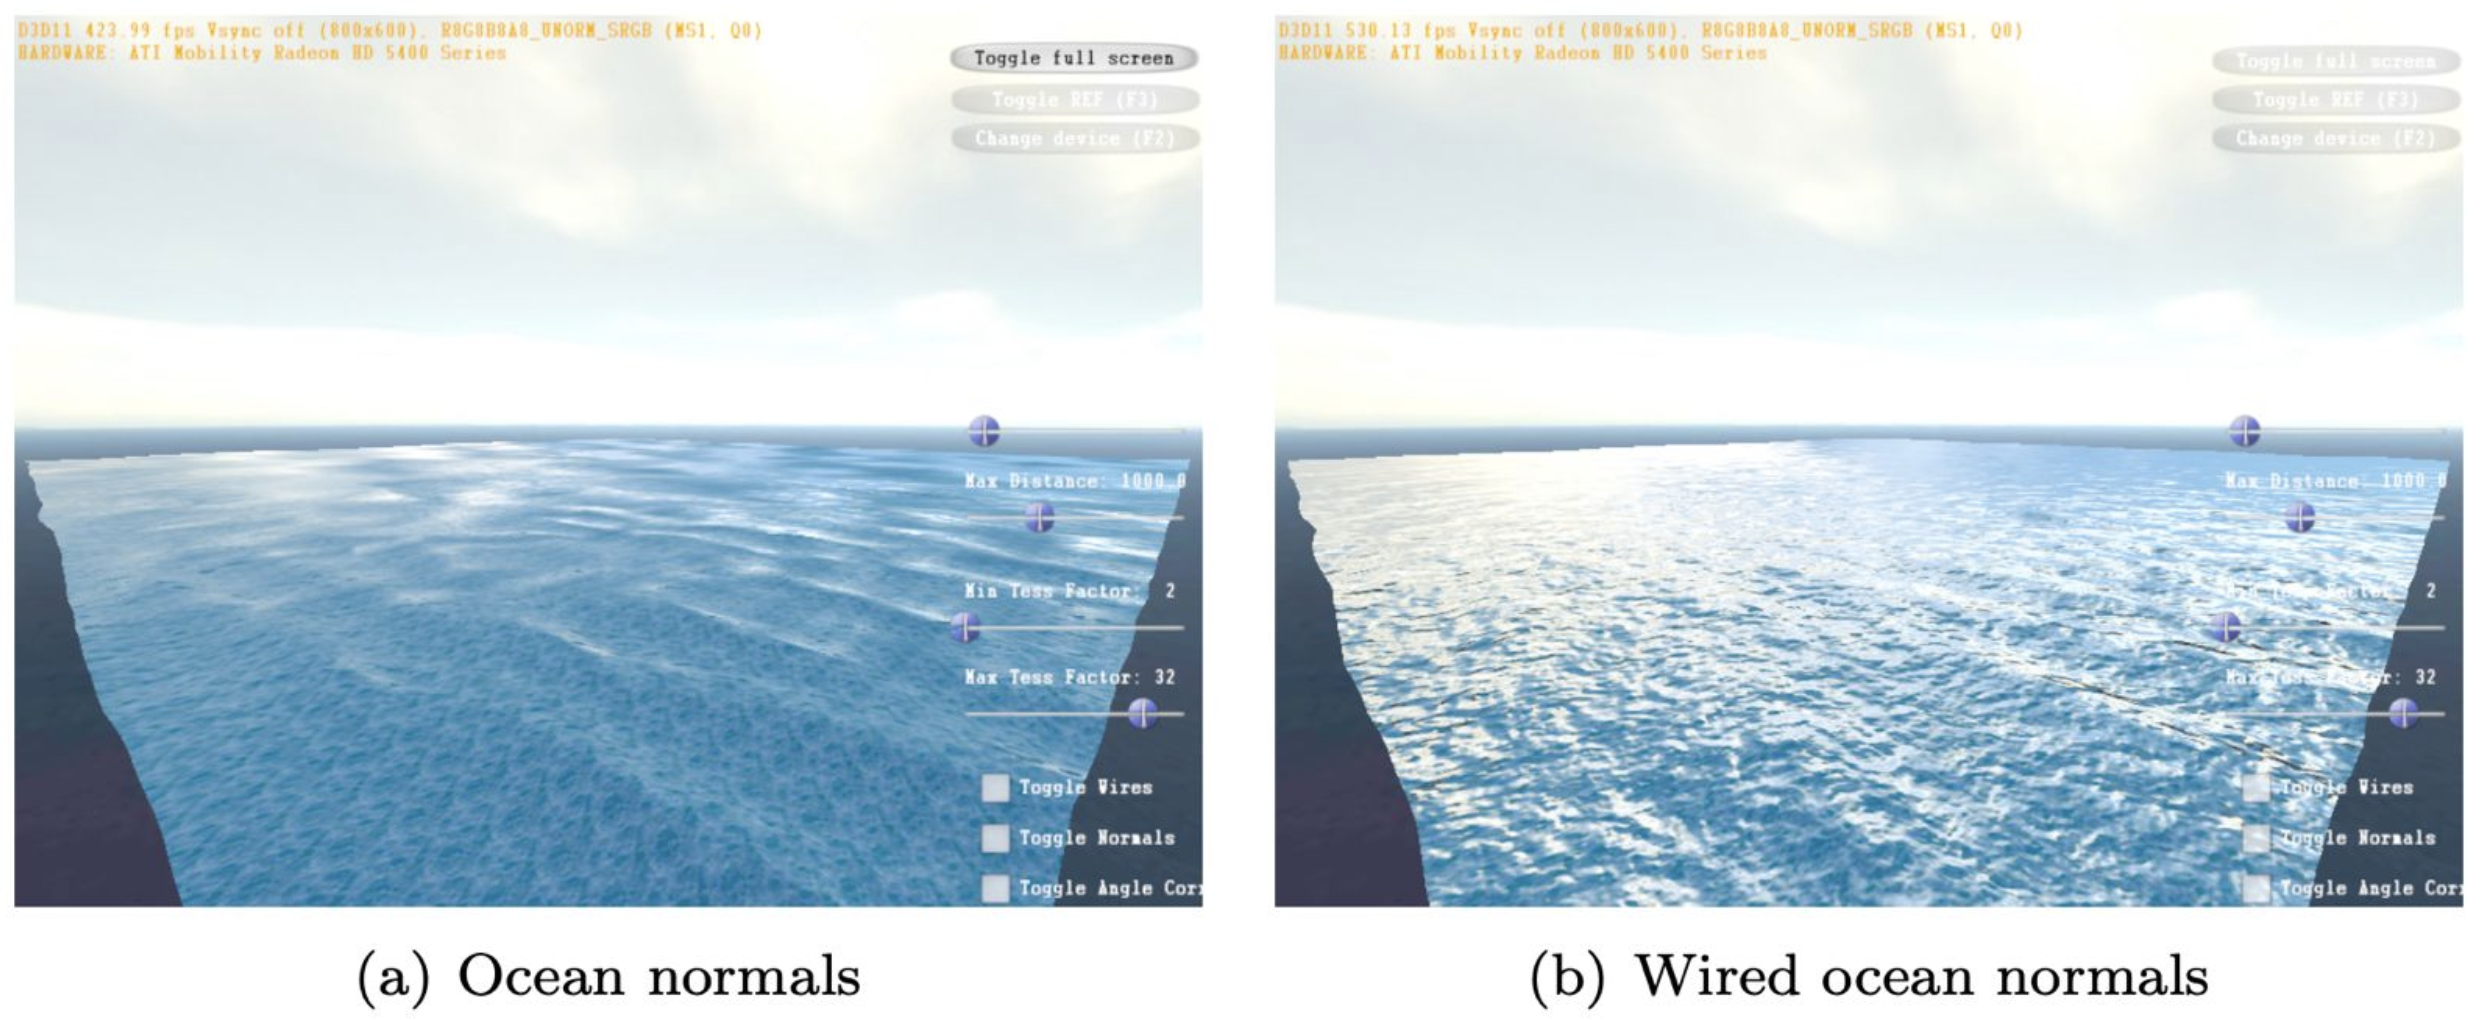
\includegraphics[width=\textwidth]{imgs/terrain-and-water-2.png}
    \end{columns}
\end{frame}


\begin{frame}{Real-time Breaking Waves for Shallow Water Simulations}
        \begin{itemize}
        \item \textbf{Objetivo:} Aprimorar simulações de águas rasas com o efeito de ondas que quebram, utilizando um modelo de campo de altura eficiente para aplicações em tempo real.
        \item \textbf{Desafio:} Simulações 3D de fluidos são computacionalmente caras para aplicações interativas.
        \item \textbf{Solução:} Combinação de simulação de campo de altura (2D) com partículas para representar ondas que quebram.
    \end{itemize}
\end{frame}

\begin{frame}{Geração de Ondas Quebrando}
    \begin{itemize}
        \item \textbf{Detecção:} Identificação de regiões com frentes de ondas íngremes onde a inclinação da altura do fluido é maior que um limiar e a velocidade do fluido se opõe ao gradiente da altura.
        \item \textbf{Critério de Detecção:} $|\nabla H(x)| > t_H$ e $\nabla H(x) \cdot u(x) < 0$, onde $t_H = p_H g \Delta t / \Delta x$.
        \item \textbf{Construção de Linhas de Onda:} Criação de linhas de pontos conectados ao longo da frente da onda.
        \item As linhas são advectadas usando a velocidade da onda e projetadas ao longo do gradiente de altura.
        \item \textbf{Geração de Patches de Fluidos:} Criação de patches de partículas conectadas ao longo da linha da onda para representar a onda quebrando.
        \item A velocidade das partículas do patch é calculada com base na velocidade da linha da onda e na energia potencial.
    \end{itemize}
\end{frame}

\begin{frame}{Demonstração}
    \begin{columns}
        \column{0.45\textwidth}
        \centering
        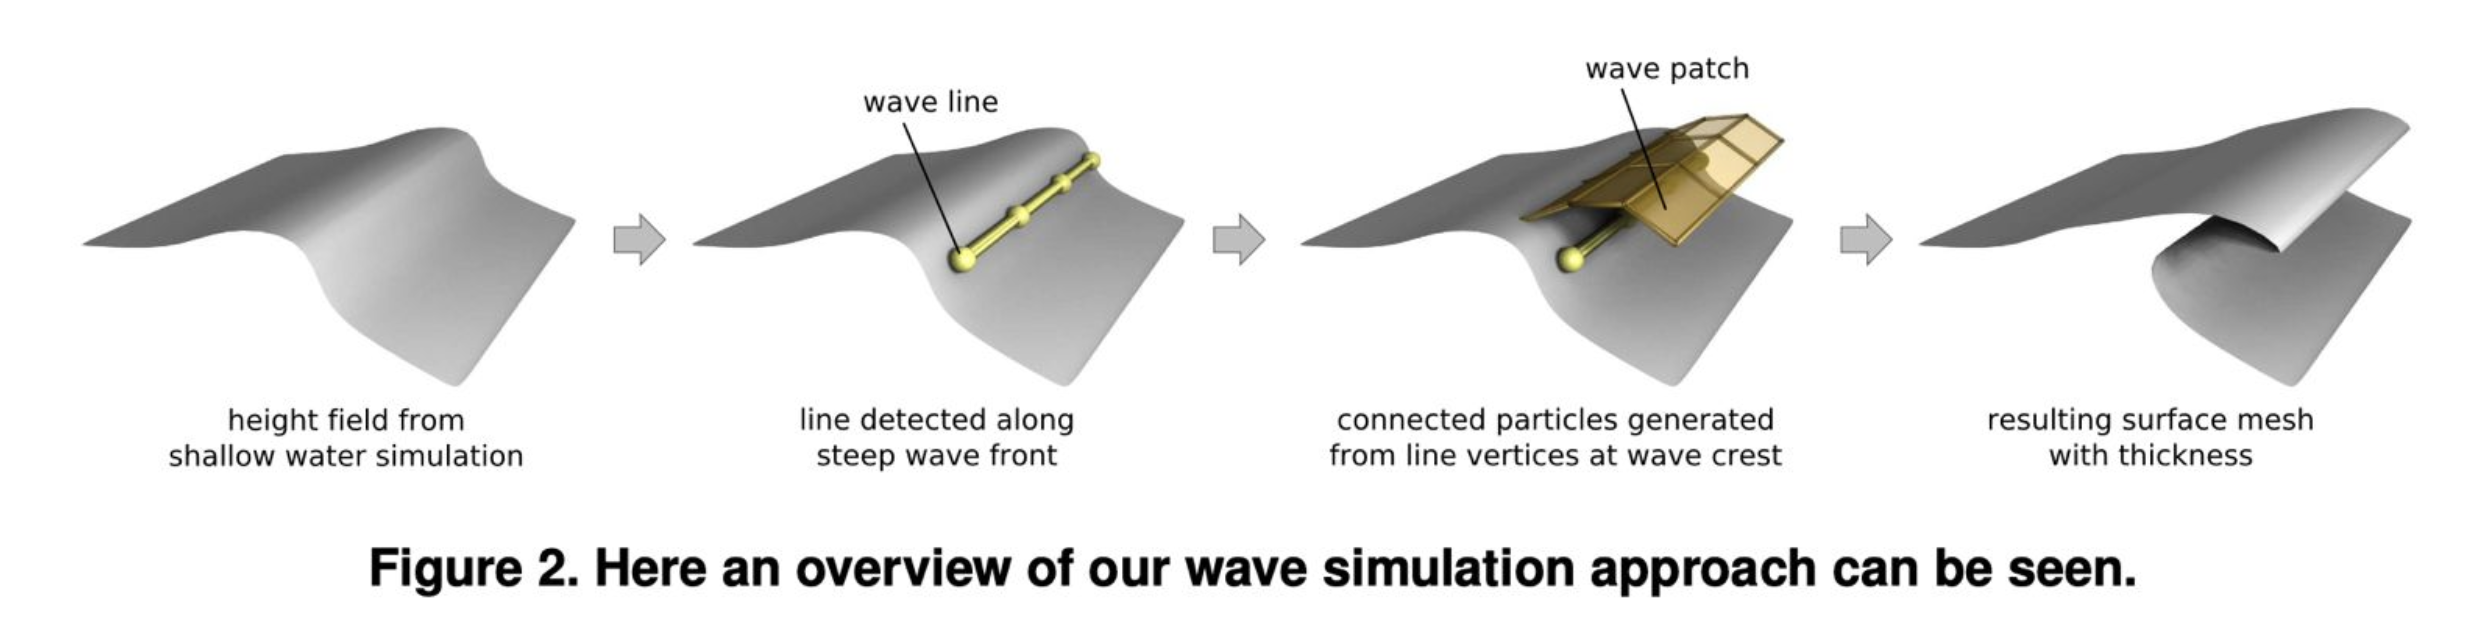
\includegraphics[width=\textwidth]{imgs/real-time-1.png}
        
        \column{0.45\textwidth}
        \centering
        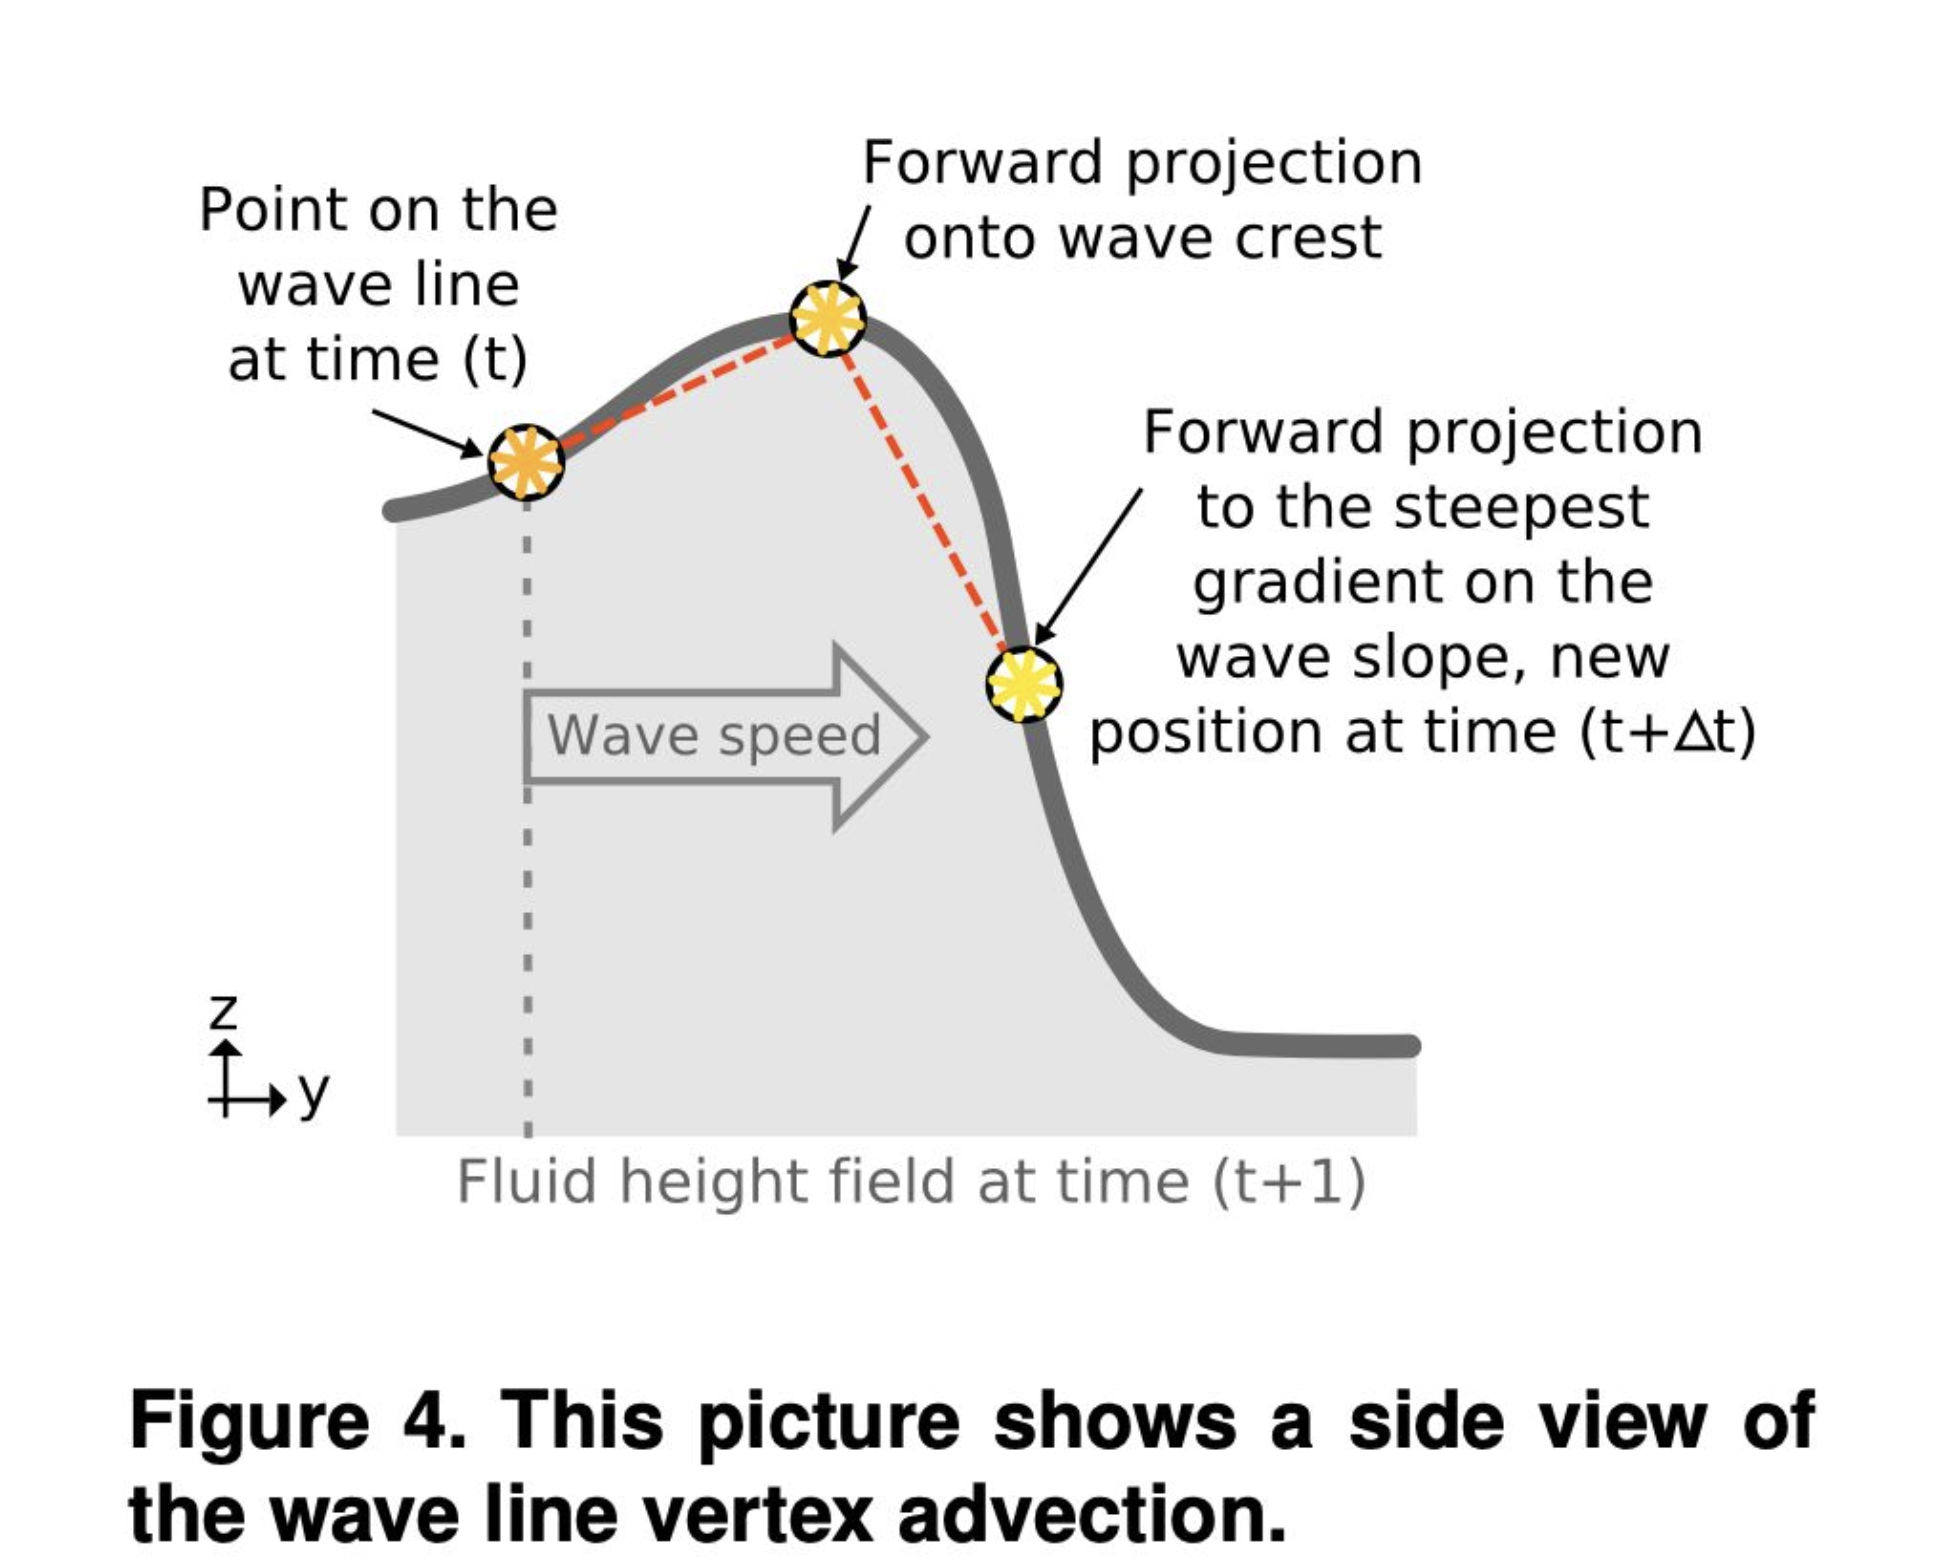
\includegraphics[width=\textwidth]{imgs/real-time-2.png}
    \end{columns}
\end{frame}

\begin{frame}{Resultados e Desempenho}
    \begin{itemize}
        \item Simulações em tempo real de ondas quebrando com taxas de quadros de 40 a 75 fps em hardware comum:
              \begin{itemize}
                  \item Intel Core 2 Duo 2.13 GHz e Nvidia Geforce 7950 GPU.
              \end{itemize}
        \item O modelo permite a criação de ondas em diversas configurações e condições.
        \item A simulação de fluidos representa cerca de 80\% do tempo de execução, enquanto a renderização e o overhead do motor gráfico consomem os 20\% restantes.
        \item Aproximadamente metade do tempo de simulação é gasto na simulação de águas rasas, e um quarto é gasto no algoritmo de simulação de ondas.
    \end{itemize}
\end{frame}

%=================================================
\section{Referências}
%=================================================
\begin{frame}[allowframebreaks]{Referências}
    \nocite{*}
    \bibliographystyle{plain}
    \bibliography{Bibliografia}
\end{frame}

\end{document}
